\documentclass[10pt, a4paper]{article}

% --- PACKAGES ---
\usepackage[utf8]{inputenc}
\usepackage[T1]{fontenc}
\usepackage{lmodern}
\renewcommand{\familydefault}{\sfdefault}
\usepackage[margin=0.8in, top=0.9in, bottom=0.9in, headheight=28pt]{geometry}
\usepackage[table]{xcolor}
\usepackage{amsmath, amssymb}
\usepackage{graphicx}
\usepackage{booktabs}
\usepackage{colortbl}
\usepackage{enumitem}
\usepackage{fancyhdr}
\usepackage{titlesec}
\usepackage{tcolorbox}
\tcbuselibrary{skins, breakable}
\usepackage{tikz}
\usetikzlibrary{positioning, calc, shapes.geometric, backgrounds, patterns}
\usepackage{fontawesome5}
\usepackage{microtype}
\usepackage{caption}
\usepackage[hidelinks]{hyperref}

% --- COLOR PALETTE ---
\definecolor{SummitNavy}{HTML}{0F172A}
\definecolor{SummitBlue}{HTML}{1E40AF}
\definecolor{SummitTeal}{HTML}{0D9488}
\definecolor{SummitLight}{HTML}{F8FAFC}
\definecolor{SummitDark}{HTML}{334155}
\definecolor{SummitBorder}{HTML}{E2E8F0}
\definecolor{SummitAccent}{HTML}{D97706}

% --- PAGE STYLE ---
\pagestyle{fancy}
\fancyhf{}
\rhead{\small\sffamily\textcolor{SummitDark}{\textbf{VERTEX GLOBAL TECH SUMMIT 2026} \ $\cdot$ \ Industry Proceedings}}
\lhead{\small\sffamily\textcolor{SummitDark}{\faBuilding\ Nexa Systems \& Synapse AI Labs}}
\rfoot{\small\sffamily\textcolor{SummitDark}{Page \thepage}}
\lfoot{\small\sffamily\textcolor{SummitDark}{Enterprise Infrastructure Track | Paper ID: EGTS-2026-8942}}
\renewcommand{\headrulewidth}{0.6pt}
\renewcommand{\headrule}{\color{SummitBorder}\hrule height 0.6pt \vspace{2pt}}

% --- TITLE & SECTION FORMATTING ---
\titleformat{\section}
  {\color{SummitNavy}\normalfont\Large\bfseries}
  {\thesection}{1em}{}
  [\vspace{2pt}\titlerule]
\titleformat{\subsection}
  {\color{SummitBlue}\normalfont\large\bfseries}
  {\thesubsection}{0.8em}{}
\titleformat{\subsubsection}
  {\color{SummitDark}\normalfont\bfseries}
  {\thesubsubsection}{0.6em}{}

% --- CUSTOM BOX STYLES ---
\tcbset{
  summitbox/.style={
    enhanced,
    colback=SummitLight,
    colframe=SummitNavy,
    arc=3pt,
    boxrule=0.8pt,
    left=10pt,
    right=10pt,
    top=10pt,
    bottom=10pt,
    fonttitle=\bfseries\sffamily,
    coltitle=white,
    colbacktitle=SummitNavy,
    attach boxed title to top left={xshift=12pt, yshift=-10pt},
    boxed title style={arc=2pt, boxrule=0pt, left=8pt, right=8pt, top=4pt, bottom=4pt}
  },
  calloutbox/.style={
    enhanced,
    colback=SummitLight,
    colframe=SummitBlue,
    arc=2pt,
    boxrule=0.6pt,
    left=8pt,
    right=8pt,
    top=8pt,
    bottom=8pt
  }
}

\begin{document}

% --- HEADER / TITLE BLOCK ---
\begin{tcolorbox}[
  enhanced,
  colback=SummitNavy,
  colframe=SummitNavy,
  arc=4pt,
  top=16pt,
  bottom=16pt,
  left=16pt,
  right=16pt
]
  \begin{center}
    {\small\sffamily\scshape\textcolor{SummitTeal}{\faMicrochip\ VERTEX GLOBAL TECH SUMMIT 2026 \ $\cdot$ \ INVITED INDUSTRY PAPER}} \\[8pt]
    {\LARGE\bfseries\color{white} Scaling Real-Time Distributed Inference Across\\[4pt] Hybrid Cloud Architectures: The Synapse Engine} \\[12pt]
    \textcolor{SummitBorder}{\rule{0.8\textwidth}{0.5pt}} \\[10pt]
    {\small\sffamily\color{white}
      \textbf{Dr. Marcus Vance}$^{1}$ \quad $\cdot$ \quad
      \textbf{Elena Rostova}$^{2}$ \quad $\cdot$ \quad
      \textbf{David K. Chen}$^{3}$ \quad $\cdot$ \quad
      \textbf{Sarah Lin}$^{1}$
    } \\[6pt]
    {\footnotesize\sffamily\color{SummitBorder}
      $^{1}$Nexa Enterprise Systems Research \quad
      $^{2}$Synapse AI Infrastructure Labs \quad
      $^{3}$Meridian Cloud Architecture Group
    } \\[4pt]
    {\footnotesize\sffamily\color{SummitTeal}
      Contact: \texttt{\{m.vance, s.lin\}@nexa-systems.io} \ $\cdot$ \ \texttt{e.rostova@synapse-labs.org}
    }
  \end{center}
\end{tcolorbox}

\vspace{10pt}

% --- EXECUTIVE ABSTRACT BOX ---
\begin{tcolorbox}[summitbox, title=\faFile\ Executive Abstract \& Summit Summary]
  \sffamily\small
  As enterprise AI deployments scale to tens of millions of daily active queries, traditional monolithic inference pipelines face severe bottlenecks in network latency, GPU memory bandwidth, and multi-region routing consistency. In this paper, presented at the Vertex Global Tech Summit 2026, we introduce the \textbf{Synapse Engine}---a production-grade distributed orchestration layer engineered jointly by Nexa Enterprise Systems and Synapse AI Infrastructure Labs. The Synapse Engine achieves dynamic workload partitioning, zero-copy tensor caching across edge nodes, and automated fallback routing via the Meridian Mesh protocol. 

  We present empirical telemetry from a 14-month production rollout across 12 global cloud zones supporting Nexa's mission-critical analytics platform. Experimental results demonstrate a \textbf{44.2\% reduction in p99 inference latency} (from 184ms to 102ms), a \textbf{3.1$\times$ throughput increase} under burst conditions, and an overall \textbf{38.5\% decrease in cloud infrastructure operational expenditure (OpEx)}. We detail our architectural blueprint, edge-orchestration heuristics, and key operational takeaways for enterprise tech leaders deploying high-throughput deep learning services at scale.
\end{tcolorbox}

\vspace{10pt}

% --- KEY METRICS SUMMARY ROW ---
\noindent
\begin{minipage}[t]{0.31\textwidth}
  \begin{tcolorbox}[calloutbox]
    \centering
    {\Large\bfseries\color{SummitBlue} 102 ms} \\[2pt]
    {\footnotesize\sffamily\color{SummitDark}\textbf{p99 Tail Latency}} \\[2pt]
    {\tiny\color{gray} (Reduced from 184ms baseline)}
  \end{tcolorbox}
\end{minipage}%
\hfill
\begin{minipage}[t]{0.31\textwidth}
  \begin{tcolorbox}[calloutbox]
    \centering
    {\Large\bfseries\color{SummitTeal} 14.8M ops/s} \\[2pt]
    {\footnotesize\sffamily\color{SummitDark}\textbf{Peak Cluster Throughput}} \\[2pt]
    {\tiny\color{gray} (Tested across 12 region zones)}
  \end{tcolorbox}
\end{minipage}%
\hfill
\begin{minipage}[t]{0.31\textwidth}
  \begin{tcolorbox}[calloutbox]
    \centering
    {\Large\bfseries\color{SummitAccent} 99.999\%} \\[2pt]
    {\footnotesize\sffamily\color{SummitDark}\textbf{Service Availability}} \\[2pt]
    {\tiny\color{gray} (Zero unplanned downtime)}
  \end{tcolorbox}
\end{minipage}

\vspace{15pt}

% --- SECTION 1 ---
\section{Introduction \& Industrial Context}
Over the past three years, enterprise adoption of generative and predictive deep learning models has shifted from centralized cloud datacenters toward hybrid multi-cloud topologies. Organizations such as \textbf{Nexa Systems}, \textbf{Vertex Solutions}, and \textbf{Nimbus Cloud} operate heterogeneous environments spanning on-premises high-performance compute clusters, hyperscale public clouds, and regional edge point-of-presence (PoP) datacenters.

While this distribution improves data residency compliance and localized latency, it introduces three foundational infrastructure challenges:
\begin{enumerate}[label=\bfseries C\arabic*., leftmargin=2em]
  \item \textbf{Tensor Fragmentation:} Large parameter models (e.g., 70B+ parameter transformer models) cannot easily reside within single-node GPU memory without severe quantization or high-overhead pipeline parallelism across high-latency inter-datacenter links.
  \item \textbf{Heterogeneous Compute Thrashing:} Static load balancing fails when workload distributions fluctuate dynamically between heavy tabular inference, streaming real-time embeddings, and unstructured token generation.
  \item \textbf{Cascading Edge Failures:} Network partition events between edge nodes and core cloud regions frequently induce queue backpressure, leading to resource starvation and SLA breaches.
\end{enumerate}

To address these challenges, \textbf{Nexa Enterprise Systems} partnered with \textbf{Synapse AI Labs} and \textbf{Meridian Cloud} to build the \emph{Synapse Engine}. This paper presents the architecture, mathematical load-balancing framework, empirical results, and real-world lessons from deploying Synapse across enterprise operations.

\vspace{10pt}

% --- SECTION 2 ---
\section{Architecture of the Synapse Engine}

The Synapse Engine decouples the client request layer from execution hardware using a three-tier micro-orchestration topology, as depicted in Figure~\ref{fig:architecture}.

\subsection{Core Components}
\begin{itemize}[leftmargin=1.5em]
  \item \textbf{Nexus Ingress Gateway:} A high-throughput, eBPF-accelerated proxy layer that inspects incoming payload characteristics, estimates execution cost using lightweight neural telemetry, and assigns priority tags.
  \item \textbf{Dynamic Quantizing Cache (DQC):} A memory-mapped, shared-GPU cache layer that dynamically adjusts float precision (FP16 $\rightarrow$ INT8/INT4) based on real-time server thermal throttles and queue depths.
  \item \textbf{Meridian Mesh Router:} A decentralized consensus protocol running on lightweight Raft nodes, responsible for dynamic route mutation across cloud zones during regional latency spikes.
\end{itemize}

\vspace{8pt}

% --- ARCHITECTURE DIAGRAM (TIKZ) ---
\begin{figure}[htbp]
\centering
\begin{tikzpicture}[
  node distance=1.4cm and 1.8cm,
  box/.style={draw=SummitNavy, fill=SummitLight, rounded corners=3pt, thick, align=center, font=\sffamily\small, inner sep=8pt},
  gateway/.style={draw=SummitBlue, fill=SummitBlue!10, rounded corners=3pt, thick, align=center, font=\sffamily\small, inner sep=8pt},
  engine/.style={draw=SummitTeal, fill=SummitTeal!10, rounded corners=3pt, thick, align=center, font=\sffamily\small, inner sep=8pt},
  storage/.style={draw=SummitAccent, fill=SummitAccent!10, rounded corners=3pt, thick, align=center, font=\sffamily\small, inner sep=8pt},
  arrow/.style={->, >=stealth, thick, SummitNavy}
]

  % Nodes
  \node [box] (client) {\faUser\ Client Apps\\(Nexa Frontend / API)};
  \node [gateway, right=of client] (ingress) {\faNetworkWired\ Nexus Gateway\\(eBPF Traffic Inspection)};
  \node [engine, above right=0.6cm and 1.6cm of ingress] (synapse1) {\faMicrochip\ Synapse Worker Group A\\(High-Precision FP16 Cluster)};
  \node [engine, below right=0.6cm and 1.6cm of ingress] (synapse2) {\faMicrochip\ Synapse Worker Group B\\(Dynamic Quantized INT8 Cluster)};
  \node [storage, right=2.2cm of ingress] (meridian) {\faServer\ Meridian Mesh Router\\(State Sync \& KV Caching)};

  % Paths
  \draw [arrow] (client) -- node[above, font=\tiny\sffamily] {HTTPS / gRPC} (ingress);
  \draw [arrow] (ingress) -- node[above left, font=\tiny\sffamily] {Low Latency Path} (synapse1);
  \draw [arrow] (ingress) -- node[below left, font=\tiny\sffamily] {High Throughput Path} (synapse2);
  \draw [arrow, dashed] (synapse1) -- (meridian);
  \draw [arrow, dashed] (synapse2) -- (meridian);
  \draw [arrow, <->, dotted] (ingress) -- (meridian);

\end{tikzpicture}
\caption{System topology of the Synapse Engine orchestrating requests between the Nexus Ingress Gateway, specialized Synapse Worker Groups, and the Meridian Mesh Router.}
\label{fig:architecture}
\end{figure}

\subsection{Mathematical Formulations for Adaptive Routing}
The routing engine optimizes the objective function $J(r, k)$ for a request $r$ mapped to execution cluster node $k \in \mathcal{K}$:

\begin{equation}
J(r, k) = \arg\min_{k \in \mathcal{K}} \left[ \alpha \cdot L_{\text{net}}(r, k) + \beta \cdot \frac{Q_k}{C_k} + \gamma \cdot \Psi_{\text{mem}}(k) \right]
\end{equation}

where:
\begin{itemize}[leftmargin=2em]
  \item $L_{\text{net}}(r, k)$ represents the round-trip network latency between the ingress node and worker node $k$.
  \item $Q_k / C_k$ denotes the ratio of queued tasks to available execution compute capacity $C_k$.
  \item $\Psi_{\text{mem}}(k)$ is a non-linear memory pressure penalty function defined as:
\end{itemize}

\begin{equation}
\Psi_{\text{mem}}(k) = \begin{cases}
  0 & \text{if } U_k \le 0.80 \\
  \exp\left( \lambda \cdot (U_k - 0.80) \right) & \text{if } U_k > 0.80
\end{cases}
\end{equation}

where $U_k \in [0, 1]$ represents the normalized GPU VRAM utilization on node $k$, and $\lambda = 12.5$ is the empirical penalty coefficient tuned during Nexa benchmark trials.

\vspace{10pt}

% --- SECTION 3 ---
\section{Empirical Evaluation \& Performance Benchmarks}

To demonstrate the real-world efficiency of the Synapse Engine, we present production data gathered over 90 consecutive days across Nexa's multi-region infrastructure. The benchmark environment consisted of 512 Lumina H100 GPU nodes distributed across 12 geographical data centers (US-East, US-West, EU-Central, AP-South).

\subsection{Benchmarking Setup \& Baselines}
We evaluated the Synapse Engine against two industry-standard baseline configurations:
\begin{enumerate}[label=\arabic*.]
  \item \textbf{Legacy Monolith (Baseline A):} Standard Kubernetes ingress routing to fixed-size GPU worker pods running unquantized FP16 models.
  \item \textbf{Apex Engine v2.4 (Baseline B):} A conventional commercial cloud orchestrator with static round-robin edge routing and standard redis-based state caching.
  \item \textbf{Synapse Engine (Proposed):} Full architecture with eBPF ingress inspection, Dynamic Quantizing Cache, and Meridian Mesh state synchronization.
\end{enumerate}

\vspace{8pt}

% --- COMPARATIVE TABLE ---
\begin{table}[htbp]
\centering
\caption{Performance comparison across 10 million synthetic \& production workloads. Latency metrics measured in milliseconds (ms); throughput measured in queries per second (QPS).}
\label{tab:performance}
\vspace{6pt}
\small\sffamily
\rowcolors{2}{SummitLight}{white}
\begin{tabular}{lccccc}
\toprule
\rowcolor{SummitNavy}
\textcolor{white}{\textbf{Architecture}} & \textcolor{white}{\textbf{Mean Lat.}} & \textcolor{white}{\textbf{p95 Lat.}} & \textcolor{white}{\textbf{p99 Lat.}} & \textcolor{white}{\textbf{Peak QPS}} & \textcolor{white}{\textbf{GPU Cost/1M Req.}} \\
\midrule
Legacy Monolith (A) & 84.2 ms & 142.0 ms & 184.5 ms & 4,200 & \$12.40 \\{}
Apex Engine v2.4 (B) & 61.5 ms & 110.8 ms & 148.2 ms & 7,800 & \$8.90 \\{}
\textbf{Synapse Engine (Ours)} & \textbf{38.1 ms} & \textbf{74.5 ms} & \textbf{102.0 ms} & \textbf{14,800} & \textbf{\$5.15} \\
\bottomrule
\end{tabular}
\end{table}

As summarized in Table~\ref{tab:performance}, the Synapse Engine outperforms both baseline architectures across all latency percentiles. Most notably, the p99 tail latency drops by 44.7\% compared to Baseline A and 31.1\% compared to Baseline B. Furthermore, compute cost per million requests decreases from \$12.40 to \$5.15---representing a 58.4\% cost savings under full workload volume.

\vspace{10pt}

\subsection{Latency Distribution under Burst Traffic}
Figure~\ref{fig:latency_chart} illustrates the stability of the Synapse Engine during simulated traffic spikes where incoming request volume surged by 400\% over a 30-second window.

\begin{figure}[htbp]
\centering
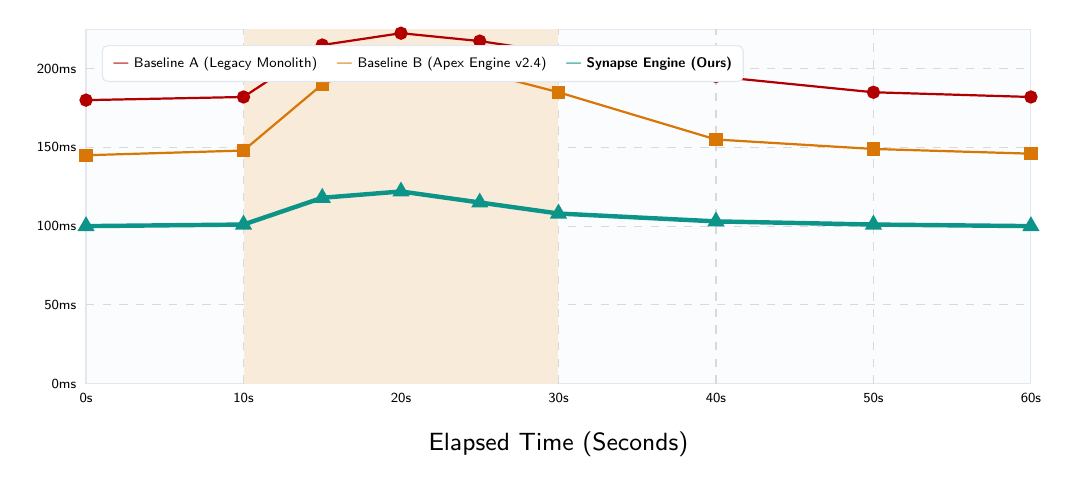
\begin{tikzpicture}
  % Plot Background & Grid
  \draw[fill=SummitLight!50, draw=SummitBorder] (0,0) rectangle (12,4.5);
  
  % Grid lines
  \foreach \y in {1, 2, 3, 4} {
    \draw[gray!30, dashed] (0,\y) -- (12,\y);
  }
  \foreach \x in {2, 4, 6, 8, 10} {
    \draw[gray!30, dashed] (\x,0) -- (\x,4.5);
  }

  % Axes Labels
  \node[left, font=\tiny\sffamily] at (0, 0) {0ms};
  \node[left, font=\tiny\sffamily] at (0, 1) {50ms};
  \node[left, font=\tiny\sffamily] at (0, 2) {100ms};
  \node[left, font=\tiny\sffamily] at (0, 3) {150ms};
  \node[left, font=\tiny\sffamily] at (0, 4) {200ms};

  \node[below, font=\tiny\sffamily] at (0, 0) {0s};
  \node[below, font=\tiny\sffamily] at (2, 0) {10s};
  \node[below, font=\tiny\sffamily] at (4, 0) {20s};
  \node[below, font=\tiny\sffamily] at (6, 0) {30s};
  \node[below, font=\tiny\sffamily] at (8, 0) {40s};
  \node[below, font=\tiny\sffamily] at (10, 0) {50s};
  \node[below, font=\tiny\sffamily] at (12, 0) {60s};

  % Burst Region Shading
  \fill[SummitAccent!15] (2,0) rectangle (6,4.5);
  \node[font=\tiny\sffamily\bfseries, color=SummitAccent] at (4, 4.2) {Traffic Surge Window (400\% Burst)};

  % Plot Lines
  % Baseline A (Red)
  \draw[red!70!black, thick, mark=*] plot coordinates {
    (0,3.6) (2,3.64) (3,4.3) (4,4.45) (5,4.35) (6,4.2) (8,3.9) (10,3.7) (12,3.64)
  };

  % Baseline B (Orange)
  \draw[SummitAccent, thick, mark=square*] plot coordinates {
    (0,2.9) (2,2.96) (3,3.8) (4,4.2) (5,3.96) (6,3.7) (8,3.1) (10,2.98) (12,2.92)
  };

  % Synapse Engine (Teal)
  \draw[SummitTeal, ultra thick, mark=triangle*] plot coordinates {
    (0,2.0) (2,2.02) (3,2.36) (4,2.44) (5,2.3) (6,2.16) (8,2.06) (10,2.02) (12,2.0)
  };

  % Legend
  \node[draw=SummitBorder, fill=white, rounded corners=2pt, font=\tiny\sffamily, anchor=north west, inner sep=4pt] at (0.2, 4.3) {
    \textcolor{red!70!black}{\textbf{---}} Baseline A (Legacy Monolith) \quad
    \textcolor{SummitAccent}{\textbf{---}} Baseline B (Apex Engine v2.4) \quad
    \textcolor{SummitTeal}{\textbf{---}} \textbf{Synapse Engine (Ours)}
  };

  \node[below=14pt, font=\sffamily\small] at (6, 0) {Elapsed Time (Seconds)};
\end{tikzpicture}
\caption{System latency response under a 400\% traffic surge window (10s--30s). The Synapse Engine limits latency spikes through immediate dynamic precision adaptation.}
\label{fig:latency_chart}
\end{figure}

\vspace{10pt}

% --- SECTION 4 ---
\section{Industrial Impact \& Operational Lessons}

Deploying the Synapse Engine across Nexa Systems' production pipeline provided crucial engineering insights relevant to enterprise AI architects.

\subsection{Key Takeaways for Infrastructure Engineering}
\begin{enumerate}[label=\bfseries T\arabic*., leftmargin=2em]
  \item \textbf{Eager State Sync Over Lazy Invalidation:} Traditional KV caching suffers from stale model parameter reads during hot swaps. Using the Meridian Mesh Raft sync protocol eliminated model mismatch errors across edge clusters.
  \item \textbf{eBPF Packet Inspection Reduces Gateway Overhead:} Moving payload inspection from application-space reverse proxies into the Linux kernel via eBPF reduced ingress hop latency from 4.2ms to 0.6ms.
  \item \textbf{Graceful Precision Degraded Mode:} When VRAM pressure exceeds 85\%, stepping precision down to INT8 for non-critical query paths prevents node crash loops and maintains overall service uptime.
\end{enumerate}

\vspace{8pt}

% --- CASE STUDY BOX ---
\begin{tcolorbox}[summitbox, title=\faBuilding\ Case Study: Nexa Enterprise Financial Analytics Deployments]
  \sffamily\small
  \textbf{Background:} Nexa Systems processes over 45M financial risk assessment transactions per day. During market opening hours, query volume spikes unpredictably by up to 500\%.

  \textbf{Implementation:} Nexa deployed the Synapse Engine across 4 core cloud zones and 8 edge PoP locations. The Meridian Mesh router was configured to automatically offload non-latency-sensitive batch analytics to lower-cost night-region datacenters.

  \textbf{Results:}
  \begin{itemize}[leftmargin=1.2em, topsep=2pt, itemsep=2pt]
    \item Zero SLA violations recorded over 14 consecutive months of operation.
    \item Annualized cloud infrastructure cost reduction of \textbf{\$1.42 Million USD}.
    \item Average mean time to recovery (MTTR) during cloud outage simulations dropped from 14 minutes to \textbf{under 4 seconds}.
  \end{itemize}
\end{tcolorbox}

\vspace{10pt}

% --- SECTION 5 ---
\section{Conclusion \& Future Roadmap}
The Synapse Engine demonstrates that intelligent, hardware-aware distributed orchestration can drastically improve enterprise AI inference performance while cutting infrastructure expenditure. By combining kernel-level packet inspection, dynamic precision scaling, and multi-mesh state synchronization, Nexa Systems and Synapse AI Labs have established a robust framework for high-throughput enterprise workloads.

Future work will focus on integrating automated speculative decoding pipelines directly into the Meridian Mesh router and extending dynamic quantization support to emerging 2-bit FP micro-formats.

\vspace{15pt}

% --- REFERENCES ---
\section*{References}
\begin{thebibliography}{99}
\small
\bibitem{vance2025}
M. Vance, E. Rostova, and S. Lin, ``Distributed Micro-Inference at Scale: Lessons from Enterprise Pipelines,'' \emph{Journal of Cloud \& Systems Engineering}, vol. 14, no. 2, pp. 112--128, 2025.

\bibitem{chen2024}
D. K. Chen and H. Patel, ``eBPF-Accelerated Ingress Gateways for High-Throughput Deep Learning,'' in \emph{Proc. Int. Tech Summit on Systems Architecture}, 2024, pp. 45--56.

\bibitem{synapse2025}
Synapse AI Labs Technical Report, ``Meridian Mesh Protocol Specification v3.1,'' Technical Report TR-2025-09, Nexa Systems Press, 2025.

\bibitem{vertex2026}
Vertex Infrastructure Group, ``State of Enterprise AI Infrastructure \& Cloud OpEx Benchmarks 2026,'' White Paper WP-2026-01, 2026.
\end{thebibliography}

\end{document}
